\documentclass[tikz,border=6pt]{standalone}

% общий стиль (подключается через TEXINPUTS)
% tikz-style.tex (общий стиль для всех TikZ-картинок)
\RequirePackage[T1,T2A]{fontenc}
\RequirePackage[utf8]{inputenc}

% Palatino-подобный шрифт (как в MathJax часто воспринимается «более вытянутым»)
\RequirePackage{txfonts}
% txfonts даёт предупреждение по кириллице (T2A/txr не определён).
% Оставляем txfonts для математики, а текстовый шрифт возвращаем на Computer Modern,
% чтобы не искать T2A/txr и убрать предупреждения.
\renewcommand{\rmdefault}{cmr}
\renewcommand{\sfdefault}{cmss}
\renewcommand{\ttdefault}{cmtt}

\RequirePackage{tikz}
\RequirePackage{xcolor}
\usetikzlibrary{calc}

% цвета
\definecolor{lightgreen}{RGB}{214,234,214}
\definecolor{darkgreen}{HTML}{0B7A0B}
\definecolor{darkred}{HTML}{DF0000}

\definecolor{midgreen}{HTML}{2E9B2E}
\definecolor{palegreen}{RGB}{235,246,235}
\definecolor{olivegreen}{HTML}{3E6B2F}

\definecolor{lightred}{RGB}{255,220,220}
\definecolor{midred}{HTML}{E04545}
\definecolor{darkred2}{HTML}{A80000}

\definecolor{lightblue}{RGB}{220,232,255}
\definecolor{midblue}{HTML}{2E5BD6}
\definecolor{darkblue}{HTML}{0B2E8A}

\definecolor{lightgray}{RGB}{240,240,240}
\definecolor{midgray}{RGB}{170,170,170}
\definecolor{darkgray}{RGB}{80,80,80}

\definecolor{vtxfill}{RGB}{86,193,255}
\definecolor{vennfill}{RGB}{220,232,255}


% единый набор стилей TikZ
\tikzset{
    lab/.style={
        font=\fontsize{24}{32}\selectfont
    }
}


\usepackage{tikz}
\usetikzlibrary{arrows.meta}

\begin{document}
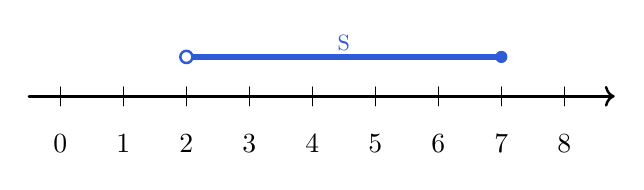
\begin{tikzpicture}[x=0.8cm,y=1cm, line cap=round, line join=round]

\draw[->, line width=0.9pt] (-0.5,0) -- (8.8,0);

\foreach \x in {0,...,8} {
  \draw (\x,0.12) -- (\x,-0.12);
  \node at (\x,-0.6) {\x};
}

\def\yS{0.50}
\def\labelscale{0.80}
\pgfmathsetlengthmacro{\labelgap}{1.2ex}

% S: (2, 7]
\draw[line width=2.2pt, color=midblue] (2,\yS) -- (7,\yS);
\draw[midblue, line width=0.9pt, fill=white] (2,\yS) circle (2.2pt);
\fill[midblue] (7,\yS) circle (2.2pt);

\node[color=midblue, font=\normalsize, scale=\labelscale] at ($(4.5,\yS)+(0,\labelgap)$) {S};

\end{tikzpicture}
\end{document}
